\documentclass[11pt,a4paper]{article}
\usepackage[utf8]{inputenc}
\usepackage[T1]{fontenc}
\usepackage[english]{babel}
\usepackage[margin=2.1cm]{geometry}
\usepackage{booktabs,array,tabularx}
\usepackage{xcolor}
\usepackage{graphicx}
\usepackage{pgfplots}
\pgfplotsset{compat=1.17}
\PassOptionsToPackage{hyphens}{url}
\usepackage[hidelinks]{hyperref}
\usepackage{enumitem}
\setlist{nosep,leftmargin=1.4em}
\emergencystretch=3em

\definecolor{impl}{HTML}{3B6EA8}
\definecolor{rev}{HTML}{8FB3DA}

\title{Sweatshop on P-Chess: the repertoire screen\\\large From openings (OPEN-005), the repertoire viewer (OPEN-006) and the repertoire editor (OPEN-007); first run of the GPT-6.1 Terra lineup, lane \texttt{repertoire}}
\author{Foreman, session \texttt{sweatshop/repertoire/2026-10-30-1830}}
\date{30 October 2026}

\begin{document}
\maketitle

\section*{Summary}

A lane run (\texttt{-Lane repertoire}) in a fresh clone at \path{.artifacts-build/lanes/repertoire},
default lineup \texttt{terra} (new on 30 October): stage 2 on \texttt{gpt-6.1-terra high} (hard
tickets on \texttt{gpt-6.1-terra xhigh}, none this run), review on \texttt{gpt-6.1-sol xhigh}.
Three \texttt{Difficulty: normal} tickets in a serial chain. Two other lanes (\texttt{analysis},
\texttt{v010}) ran at the same time in their own clones. Launch at 18:30, last merge at 19:29.

\begin{itemize}
  \item \textbf{Produced:} OPEN-005, OPEN-006 and OPEN-007 merged on the session,
        \texttt{Verdict: Approve}, all \texttt{Review: agent}. Session PR
        \href{https://github.com/Laginho/P-Chess/pull/25}{\#25}; checks \texttt{test} and
        \texttt{windows-export} green. Gate 280 passed, 0 failed, 4 Lc0 skips (271 on the
        session before OPEN-005).
  \item \textbf{Cost:} \textbf{\$4.55} at API list price over the 4 priced stages (all reviews,
        \texttt{gpt-6.1-sol xhigh}); the 4 \texttt{gpt-6.1-terra high} stages log \texttt{?}
        because the driver's \texttt{\$CodexPrices} has no Terra row. Codex quota: 4 points of
        the weekly window (Terra 1, Sol 2, outside stages 1, each $\pm$1), shared with the
        two concurrent lanes.
  \item \textbf{What went wrong:} OPEN-006's first handoff was parked: Terra wrote the
        \texttt{Gate evidence:} path with its backslashes eaten, and the driver ended the run.
        The foreman repaired the line and relaunched. OPEN-007 was reopened once with four
        implementer findings (one P1).
  \item \textbf{Provisional verdict:} Terra is fast (median 7.5~min per stage 2 against Sol
        high's 11) and keeps test-first discipline, but it slipped on handoff hygiene in 2 of 3
        tickets and on UI test realism in the third. Three reviews is an anecdote.
\end{itemize}

\section*{What was done}

\textbf{OPEN-005}: a repertoire screen opens from setup's repertoire controls. It lists the
saved repertoires and offers Import PGN or \emph{From openings}. From openings shows the opening
catalog as a tree of names with checkboxes; you pick White or Black and a name, and the lines
are saved through the same PGN import path, so My repertoire mode, ``check my moves'' and the
review badges treat them as an imported repertoire. Empty selection or blank name is refused.
Main files \path{ui/repertoire_screen.gd}, \path{ui/opening_picker.gd},
\path{bot/repertoire.gd} (\texttt{save\_openings}).

\textbf{OPEN-006}: the repertoire screen gains a board beside the line list, oriented to the
repertoire's colour. Clicking a line shows its final position and last move; the arrow keys step
through it and stop at both ends. Lines are named from the catalog where they match, otherwise
shown as moves. Main file \path{ui/repertoire_screen.gd}. Not reopened; its only problem was
the handoff line (see Driver and runtime issues).

\textbf{OPEN-007}: an Edit button opens an editor from the selected line's final position or
from the start. Playing a legal move extends the line or adds a branch; a tree list shows the
branches; right-click deletes a move and everything after it; Save writes the usual format,
Cancel discards. Main files \path{ui/repertoire_editor.gd} and \path{bot/repertoire.gd}.
Reopened once, four findings: the Edit button shipped disabled and nothing enabled it
(\path{ui/repertoire_screen.tscn}); right-click rebuilt the tree inside Godot's mouse-selection
callback, leaving a stale tree and board (\path{ui/repertoire_editor.gd}); the editor used a
normal \texttt{Game}, so insufficient-material adjudication refused some legal moves (same
file); and Terra's own annotation-preservation addition moved an imported variation comment
onto the previous move on save (\path{bot/repertoire.gd}). The cause of the first two was the
same: the tests emitted the signal directly instead of dispatching input. All four were fixed
test-first in one pass and approved with no new finding.

\section*{Timeline}

\begin{tabularx}{\linewidth}{@{}lX@{}}
\toprule
18:30 & Clone of \texttt{origin} at \texttt{eea8c16}; launch, pid 27856; \texttt{main}'s CI on \texttt{eea8c16} still running (later green). \\
18:41 & OPEN-005 to review (Terra, 10~min). \\
18:47 & OPEN-005 merged, 0 findings. OPEN-006 stage 2. \\
18:52 & OPEN-006 parked: \texttt{failed (incomplete handoff)}, ``Illegal characters in path''. Driver ends, PR \#25 opened (1 ticket). \\
18:54 & Foreman repairs the evidence path, restores \texttt{to-review} (\texttt{7322f84}). \\
18:55 & Relaunch, pid 26444. \\
19:00 & OPEN-006 merged, 0 findings. OPEN-007 stage 2. \\
19:08 & OPEN-007 to review (Terra, 7~min). \\
19:15 & OPEN-007 reopened, 4 findings. Stage 2 again. \\
19:23 & OPEN-007 to review (Terra, 8~min). \\
19:29 & OPEN-007 merged, 0 new findings; nothing left in the lane; PR \#25 updated (3 tickets). \\
\bottomrule
\end{tabularx}

\section*{Per stage}

{\small
\begin{tabularx}{\linewidth}{@{}llllrrrrrX@{}}
\toprule
When & Ticket & Stage & Model & Min & In & Cache & Out & Cost & Outcome \\
\midrule
18:41 & OPEN-005 & impl & terra high & 10 & 5.0M & 98\% & 13k & ? & to-review \\
18:47 & OPEN-005 & review & sol xhigh & 6 & 2.9M & 95\% & 15k & 1.01 & merged \\
18:52 & OPEN-006 & impl & terra high & 5 & 1.9M & 96\% & 7k & ? & handoff failed \\
19:00 & OPEN-006 & review & sol xhigh & 5 & 3.0M & 96\% & 13k & 0.93 & merged \\
19:08 & OPEN-007 & impl & terra high & 7 & 3.1M & 98\% & 12k & ? & to-review \\
19:15 & OPEN-007 & review & sol xhigh & 7 & 4.4M & 96\% & 25k & 1.49 & reopened \\
19:23 & OPEN-007 & impl & terra high & 8 & 4.2M & 98\% & 12k & ? & to-review \\
19:29 & OPEN-007 & review & sol xhigh & 6 & 3.3M & 95\% & 18k & 1.12 & merged \\
\midrule
 & & & & 54 & 27.8M & & 115k & 4.55+? & \\
\bottomrule
\end{tabularx}
}

\begin{center}
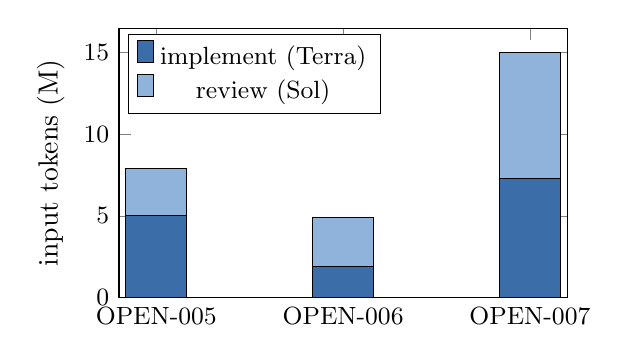
\begin{tikzpicture}
\begin{axis}[ybar stacked, bar width=22pt, width=0.6\linewidth, height=5cm,
  symbolic x coords={OPEN-005,OPEN-006,OPEN-007},
  xtick=data, ylabel={input tokens (M)}, ymin=0, legend style={at={(0.02,0.98)},anchor=north west,font=\small},
  tick label style={font=\small}]
\addplot[fill=impl] coordinates {(OPEN-005,5.0) (OPEN-006,1.9) (OPEN-007,7.3)};
\addplot[fill=rev] coordinates {(OPEN-005,2.9) (OPEN-006,3.0) (OPEN-007,7.7)};
\legend{implement (Terra), review (Sol)}
\end{axis}
\end{tikzpicture}
\end{center}

The chart is input tokens, not dollars: Terra's stages are unpriced. Wasted: OPEN-006's first
stage 2 (1.9M in) was complete work parked on one corrupt line; it was reused, not redone, so
the waste is the driver restart. OPEN-007's first round (3.1M implement + 4.4M review) is the
cost of the reopen.

\section*{Comparison with previous runs}

From \texttt{run-log.md}: the 27 October \texttt{sol} QA lane cost \$5.86 for three hard tickets
on \texttt{gpt-6.1-sol xhigh} (11--17~min per stage 2, 0 findings). Over all its P-Chess runs,
\texttt{gpt-6.1-sol high} ran 21 stage 2s, 21 to review, 0 failed, median 11~min, mean \$0.82.
This run's Terra stage 2s took 5--10~min (median 7.5) on similar token volumes (1.9--5.0M in,
7--13k out). Reviews cost about the same as before (\$0.93--1.49 against \$0.75--0.79 on 27
October; the dearest one is the reopening review, the longest report). Three tickets plus one
reopen cost \$4.55 for reviews alone; Terra's share is unknown until it is priced.

\section*{Observations per model}

\begin{itemize}
  \item \textbf{gpt-6.1-terra high, stage 2} (4 stages): test-first every time, with a
        \texttt{test:} commit and a recorded red run before each production commit (OPEN-007:
        four red$\to$green cycles, including a mutation check for subtree deletion; the reopen
        fix: one test/fix pair per finding). Small diffs that reuse existing paths
        (\texttt{save\_openings} goes through \texttt{import\_pgn}). Commits small, conventional,
        ticket-tagged, test/production split kept. It never asked the proxy, never hit a gate
        failure, and disclosed manual acceptance honestly.
        Weak spots: \emph{handoff hygiene}. OPEN-005 rewrote the ticket's non-ASCII as mojibake
        (the section sign became \texttt{Â} plus the sign); the review copy fixed it silently.
        OPEN-006 wrote the evidence path through an escape-processing writer, which parked the
        ticket. And \emph{UI test realism}: OPEN-007's tests emitted \texttt{pressed} and
        \texttt{item\_mouse\_selected} directly, so two P-level defects passed the tests. It also
        added unrequested annotation preservation, which brought one of the four findings.
  \item \textbf{gpt-6.1-sol xhigh, review} (4 stages, 5--7~min): each review verified the
        red/green order, reused the gate receipt after checking its hash and code, and ran its
        own headless probe through real input dispatch (17, 15, 12 and 15 checks). The reopening
        review found all four defects at once; the re-review raised nothing new (no drip-feed).
        No production code written in review, so no round-0 rows.
\end{itemize}

\section*{Driver and runtime issues}

\begin{enumerate}
  \item \texttt{\$CodexPrices} has no \texttt{gpt-6.1-terra} row: every Terra stage logs
        \texttt{?}, so the lineup's cost cannot be compared yet.
  \item OPEN-006: the handoff check threw ``Illegal characters in path'' on a
        \texttt{Gate evidence:} line whose backslashes were gone (one became a backspace
        character). Parked as \texttt{failed (incomplete handoff), blocked}; with nothing else
        runnable (OPEN-007 depended on it) the driver ended. The foreman verified the receipt
        (exit 0, log hash, code \texttt{84cfd26} = the feat commit), fixed the line on the ticket
        branch, restored \texttt{to-review} on the session and relaunched. Logged as an
        \texttt{automatic-recovery}.
  \item Codex sessions could not reach the proxy (``unreachable; the driver asks for them''), as
        on earlier runs; no stage asked, so it did not matter.
  \item Shutdown 1.0--1.8~s per stage; no crash, no timeout.
\end{enumerate}

\section*{Recommendations}

\begin{enumerate}
  \item Add a \texttt{gpt-6.1-terra} row to \texttt{\$CodexPrices} from OpenAI's pricing page
        before the next Terra run; until then the scoreboard cannot compare cost.
  \item Have the driver's handoff check say which line is bad, or have \texttt{gate-evidence.ps1}
        write the \texttt{Gate evidence:} line itself instead of the stage model typing the path.
        Terra corrupted ticket text in two of three tickets; Sol has no such failure in 30
        P-Chess stage 2s.
  \item For UI tickets, ask in the ticket's test list for tests that dispatch input
        (\texttt{Input.parse\_input\_event}) rather than emit signals: the reviewer's probes did
        this and found the two P-level defects.
  \item Keep Terra as default for \texttt{normal} tickets for now, and judge it again after ten
        reviews: scoreboard row \texttt{gpt-6.1-terra high} $\rightarrow$
        \texttt{gpt-6.1-sol xhigh}, 3 reviews, 1 reopened (33\%), S2 rate 33\% --- an
        anecdote, against \texttt{gpt-6.1-sol high} $\rightarrow$ \texttt{gpt-6.1-sol xhigh},
        18 reviews, 22\%.
\end{enumerate}

\section*{Human debt and proxy decisions}

No \texttt{Débito humano:} lines and no \texttt{Proxy decided} or \texttt{Proxy escalated} line
in this run's tickets.

\section*{Reopen attribution}

Labelled by the foreman (opus-5.5); the reviewer was \texttt{gpt-6.1-sol xhigh}, so no
self-judging. Rows appended to \path{.scratch/reopen-attribution.md}.

{\small\noindent
\begin{tabularx}{\linewidth}{@{}>{\raggedright\arraybackslash}p{1.6cm}X>{\raggedright\arraybackslash}p{2.7cm}X@{}}
\toprule
Ticket (round) & Finding & Label & Why \\
\midrule
OPEN-007 (1) & Edit button disabled, editor unreachable by click & S2-explícito/\allowbreak código & criterion 1; test emitted \texttt{pressed} directly \\
OPEN-007 (1) & Right-click rebuilds the tree in the selection callback; stale tree and board & S2-explícito/\allowbreak código & criterion 4; test emitted the signal directly \\
OPEN-007 (1) & Insufficient-material adjudication refuses legal editor moves & S2-explícito/\allowbreak código ? & criterion 2; borderline edge case \\
OPEN-007 (1) & Save moves an imported variation comment to the previous move & S2-implícito ? & regression of stage 2's own addition \\
\bottomrule
\end{tabularx}
}

Totals: S2-explícito/código 3, S2-implícito 1, S1 0, S3-ruído 0. No review miss, no
review-induced churn, no fix made in review. No session-review, release-audit or post-release
finding has been reported for this lane.

\section*{Scoreboard}

\texttt{scoreboard.ps1} over the ClassyCall, EasyMath, PhysiSyst, SIGAA-ME and SynchroNice main
checkouts, plus this lane's clone in place of P-Chess's main checkout (same merged run log; the
clone's session branch holds this run's attribution rows, which reach \texttt{main} with this
report). New rows: implementer \texttt{gpt-6.1-terra high}, 4 stage runs, 3 to review, 1 failed,
median 8~min, cost \texttt{?}; pair \texttt{gpt-6.1-terra high} $\rightarrow$
\texttt{gpt-6.1-sol xhigh}, 3 reviews, 1 reopened, S2 rate 33\% (anecdote, under 10 reviews).
Automatic recoveries 88 $\to$ 89. The other P-Chess rows did not move since the 27 October
report.

{\tiny
\begin{verbatim}
| Implementer | Stage runs | To review | Failed | Asked | Median min to review | Cost |
|---|---|---|---|---|---|---|
| gpt-6.1-sol high | 64 | 59 | 0 | 5 | 9m | $49.27 (64/64 priced) |
| opus-5.5 medium | 3 | 2 | 1 | 0 | 6m | $4.79 (3/3 priced) |
| opus-5.5 | 7 | 4 | 0 | 3 | 14m | $15.12 (7/7 priced) |
| gpt-6-luna max | 89 | 61 | 10 | 18 | 17m | $4.91 (85/89 priced) |
| sonnet-5.5 high | 2 | 2 | 0 | 0 | 7m | $3.77 (2/2 priced) |
| gpt-6-astra high | 1 | 0 | 0 | 1 | - | $3.92 (1/1 priced) |
| opus-5.5 xhigh | 18 | 14 | 4 | 0 | 12m | $91.78 (18/18 priced) |
| gpt-6.1-sol max | 6 | 5 | 0 | 1 | 24m | $12.12 (6/6 priced) |
| gpt-6-sol xhigh | 1 | 1 | 0 | 0 | 9m | $0.40 (1/1 priced) |
| fable | 1 | 1 | 0 | 0 | 11m | ? |
| gpt-6-luna | 8 | 4 | 4 | 0 | 37m | ? |
| gpt-6-sol | 6 | 5 | 1 | 0 | 17m | ? |
| gpt-5.6-sol | 5 | 4 | 1 | 0 | 17m | ? |
| gpt-6-astra | 18 | 11 | 6 | 1 | 8m | ? |
| sonnet | 5 | 3 | 2 | 0 | 14m | $10.53 (4/5 priced) |
| sonnet-5 xhigh | 11 | 6 | 2 | 3 | 8m | $18.09 (11/11 priced) |
| haiku-5.5 high | 2 | 0 | 2 | 0 | - | $1.00 (2/2 priced) |
| opus-5.5 high | 20 | 13 | 6 | 1 | 6m | $37.46 (20/20 priced) |
| gpt-6.1-sol xhigh | 9 | 9 | 0 | 0 | 12m | $9.84 (9/9 priced) |
| gpt-6.1-terra high | 4 | 3 | 1 | 0 | 8m | ? |

| Implementer | Reviewer | Reviews | Reopened | Reopen rate | Reopened for S2 | S2 rate | Unclassified | Fixed in review for S2 |
|---|---|---|---|---|---|---|---|---|
| gpt-6.1-sol high | gpt-6.1-sol max | 38 | 12 | 32% | 9 | >=24% | 2 | 1 |
| opus-5.5 medium | gpt-6.1-sol max | 2 | 1 | 50% | 0 | >=0% | 1 | 0 |
| opus-5.5 | opus-5.5 | 4 | 0 | 0% | 0 | 0% | 0 | 0 |
| gpt-6-luna max | opus-5.5 high | 18 | 1 | 6% | 1 | 6% | 0 | 0 |
| gpt-6-luna max | gpt-6-sol max | 43 | 23 | 53% | 22 | 51% | 0 | 0 |
| ? | gpt-6-sol max | 1 | 0 | 0% | 0 | 0% | 0 | 0 |
| sonnet-5.5 high | gpt-6-sol max | 2 | 1 | 50% | 1 | 50% | 0 | 0 |
| opus-5.5 xhigh | gpt-6.1-sol max | 6 | 3 | 50% | 3 | 50% | 0 | 0 |
| ? | gpt-6.1-sol max | 1 | 0 | 0% | 0 | 0% | 0 | 0 |
| gpt-6.1-sol max | gpt-6.1-sol max | 4 | 1 | 25% | 1 | 25% | 0 | 0 |
| gpt-6-sol xhigh | gpt-6-astra high | 1 | 0 | 0% | 0 | 0% | 0 | 0 |
| fable | fable | 1 | 1 | 100% | 0 | >=0% | 1 | 0 |
| ? | opus | 1 | 0 | 0% | 0 | 0% | 0 | 0 |
| gpt-6-luna | gpt-6-sol | 4 | 4 | 100% | 0 | >=0% | 4 | 0 |
| gpt-6-sol | gpt-5.6-sol | 5 | 4 | 80% | 0 | >=0% | 4 | 0 |
| gpt-5.6-sol | gpt-6-astra | 4 | 3 | 75% | 0 | >=0% | 3 | 0 |
| gpt-6-astra | gpt-5.6-sol | 11 | 5 | 45% | 0 | >=0% | 5 | 0 |
| sonnet | opus | 3 | 1 | 33% | 1 | 33% | 0 | 0 |
| sonnet-5 xhigh | opus-5.5 xhigh | 5 | 0 | 0% | 0 | 0% | 0 | 0 |
| ? | opus-5.5 xhigh | 4 | 1 | 25% | 1 | 25% | 0 | 0 |
| opus-5.5 xhigh | opus-5.5 xhigh | 7 | 0 | 0% | 0 | 0% | 0 | 0 |
| opus-5.5 high | opus-5.5 xhigh | 10 | 2 | 20% | 2 | 20% | 0 | 3 |
| gpt-6.1-sol high | gpt-6.1-sol xhigh | 18 | 4 | 22% | 4 | 22% | 0 | 0 |
| gpt-6.1-sol xhigh | gpt-6.1-sol xhigh | 9 | 1 | 11% | 1 | 11% | 0 | 1 |
| gpt-6.1-terra high | gpt-6.1-sol xhigh | 3 | 1 | 33% | 1 | 33% | 0 | 0 |
| ? | gpt-6.1-sol xhigh | 1 | 0 | 0% | 0 | 0% | 0 | 0 |

| Implementer -> Reviewer | Rounds | S2 explicit code | S2 explicit test | S2 implicit | S1 | S3 noise |
|---|---|---|---|---|---|---|
| gpt-6-astra medium -> gpt-6.1-sol max | 8 | 11 | 1 | 4 | 1 | 0 |
| gpt-6.1-sol-fast high -> gpt-6.1-sol-fast max | 2 | 2 | 0 | 0 | 0 | 0 |
| gpt-6.1-sol-fast max -> gpt-6.1-sol-fast max | 6 | 2 | 0 | 3 | 1 | 0 |
| gpt-6.1-sol high -> gpt-6.1-sol max | 26 | 16 | 4 | 23 | 1 | 0 |
| gpt-6-luna max -> opus-5.5 high | 1 | 1 | 1 | 0 | 1 | 0 |
| gpt-6-luna max -> gpt-6-sol max | 23 | 31 | 3 | 23 | 12 | 15 |
| sonnet-5.5 high -> gpt-6-sol max | 1 | 3 | 0 | 2 | 0 | 0 |
| opus-5.5 xhigh -> gpt-6.1-sol max | 3 | 3 | 0 | 2 | 1 | 0 |
| gpt-6.1-sol max -> gpt-6.1-sol max | 5 | 7 | 0 | 5 | 0 | 0 |
| haiku-5.5 high -> gpt-6.1-sol max | 3 | 3 | 1 | 5 | 1 | 0 |
| gpt-6.1-sol high -> gpt-6.1-sol xhigh | 53 | 53 | 4 | 23 | 3 | 0 |
| gpt-6.1-sol max -> gpt-6.1-sol xhigh | 2 | 0 | 0 | 3 | 0 | 0 |
| opus-5.5 high -> opus-5.5 xhigh | 8 | 7 | 0 | 3 | 0 | 0 |
| gpt-6.1-sol xhigh -> gpt-6.1-sol xhigh | 3 | 4 | 0 | 1 | 0 | 0 |
| opus-5.5 high -> gpt-6.1-sol xhigh | 1 | 2 | 0 | 0 | 0 | 0 |
| sonnet-5.5 high -> gpt-6.1-sol max | 3 | 5 | 0 | 2 | 3 | 0 |
| sonnet-5.5 xhigh -> gpt-6.1-sol max | 3 | 7 | 0 | 3 | 2 | 0 |
| sonnet-5.5 high -> opus-5.5 xhigh | 3 | 1 | 2 | 0 | 0 | 0 |
| gpt-6-astra medium -> gpt-6-astra xhigh | 1 | 1 | 0 | 0 | 0 | 0 |
| fable -> ? | 4 | 5 | 1 | 3 | 1 | 0 |
| sonnet -> ? | 10 | 3 | 6 | 9 | 3 | 2 |
| opus -> ? | 1 | 3 | 0 | 0 | 0 | 0 |
| sonnet? -> ? | 11 | 3 | 4 | 12 | 3 | 5 |
| sonnet -> opus | 1 | 1 | 1 | 0 | 0 | 0 |
| gpt-6-astra low -> gpt-6.1-sol max | 1 | 2 | 0 | 1 | 0 | 0 |
| gpt-6.1-terra high -> gpt-6.1-sol xhigh | 1 | 3 | 0 | 1 | 0 | 0 |

Evidence coverage: legacy flags and absent records are unknown, not zero defects or zero interventions.
| Discovery | Recorded findings | Earlier review miss (yes / known) | Review-induced churn (yes / known) |
|---|---|---|---|
| ticket-review | 368 | 5 / 173 | 1 / 175 |
| session-review | 28 | 22 / 24 | 0 / 27 |
| release-audit | 2 | 2 / 2 | 0 / 2 |
Runtime completion to process exit: 218.643s total over 181 measured stages; 333 unmeasured.
| Intervention | Recorded events |
|---|---|
| human-rescue | 30 |
| automatic-recovery | 89 |
| proxy-decision (unknown) | 37 |
| routine-approval | 18 |
| proxy-decision (gpt-6-astra high, fallback) | 58 |
| proxy-decision (opus) | 42 |
| proxy-decision (supervisor) | 12 |
\end{verbatim}
}

\section*{Pending for the human}

\begin{enumerate}
  \item OPEN-005: build a Caro-Kann repertoire as Black from names; play it in My repertoire mode.
  \item OPEN-006: open a repertoire, click a line, step with the physical arrow keys; check the
        layout and last-move highlight.
  \item OPEN-007: add a branch to an imported repertoire, delete a sub-line, save, play it in My
        repertoire mode.
  \item Review and merge session PR \#25, then tell the \texttt{analysis} and \texttt{v010}
        foremen to sync.
\end{enumerate}

\end{document}
